\begin{frame}
  \frametitle{Principal components analysis (PCA)}
  %% \framesubtitle{}

  \begin{itemize}
  \item We want to project the data points to a lower-dimensional subspace,
    but preserve distances as well as possible
  \item<2-> Insight 1: variance = average squared distance
    \[
    \frac{1}{k(k-1)} \sum_{i=1}^k \sum_{j=1}^k \norm{\vx[i] - \vx[j]}^2
    = \frac{2}{k-1} \sum_{i=1}^k \norm{\vx[i]}^2 = 2\sigma^2
    \]
  \item<3-> Insight 2: orthogonal projection always reduces distances\\
    \so difference in squared distances = loss of variance
  \item<4-> If we reduced the data set to just a single dimension,
    which dimension would still have the highest variance?
  \item<4-> Mathematically, we project the points onto a line through the origin
    and calculate one-dimensional variance on this line
    \begin{itemize}
    \item we'll see in a moment how to compute such projections
    \item but first, let us look at a few examples
    \end{itemize}
  \end{itemize}
\end{frame}

\begin{frame}<beamer:1-6| handout:1-3>[c]
  \frametitle{Projection and preserved variance: examples}
  %% \framesubtitle{}

  \begin{center}
    \only<beamer:1| handout:0>{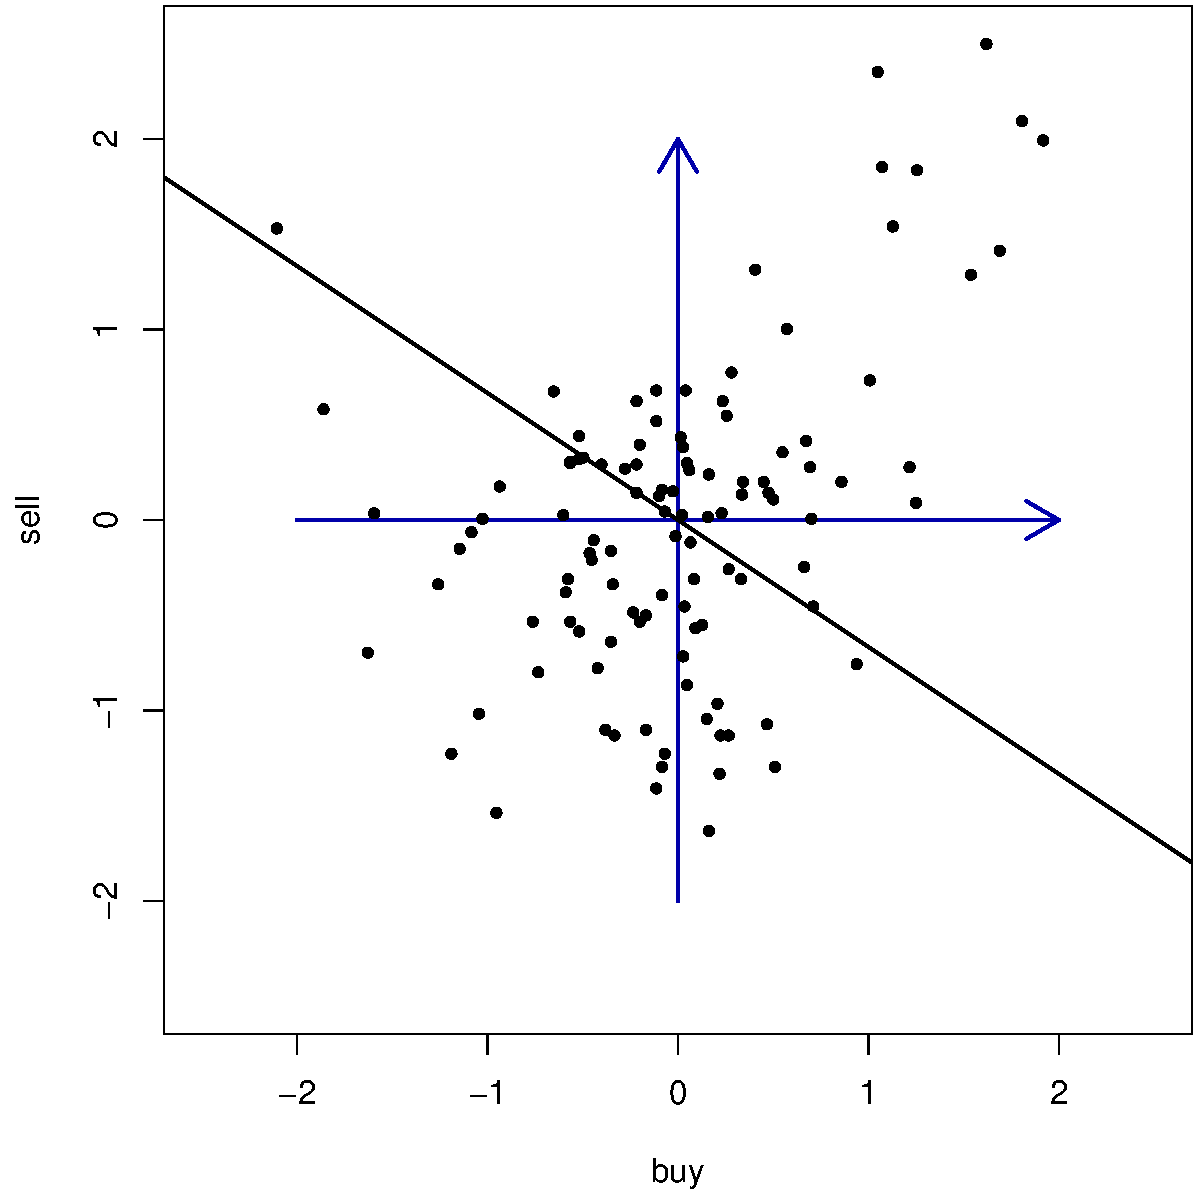
\includegraphics[width=7cm]{img/3_buy_sell_1_axis}}%
    \only<beamer:2| handout:1>{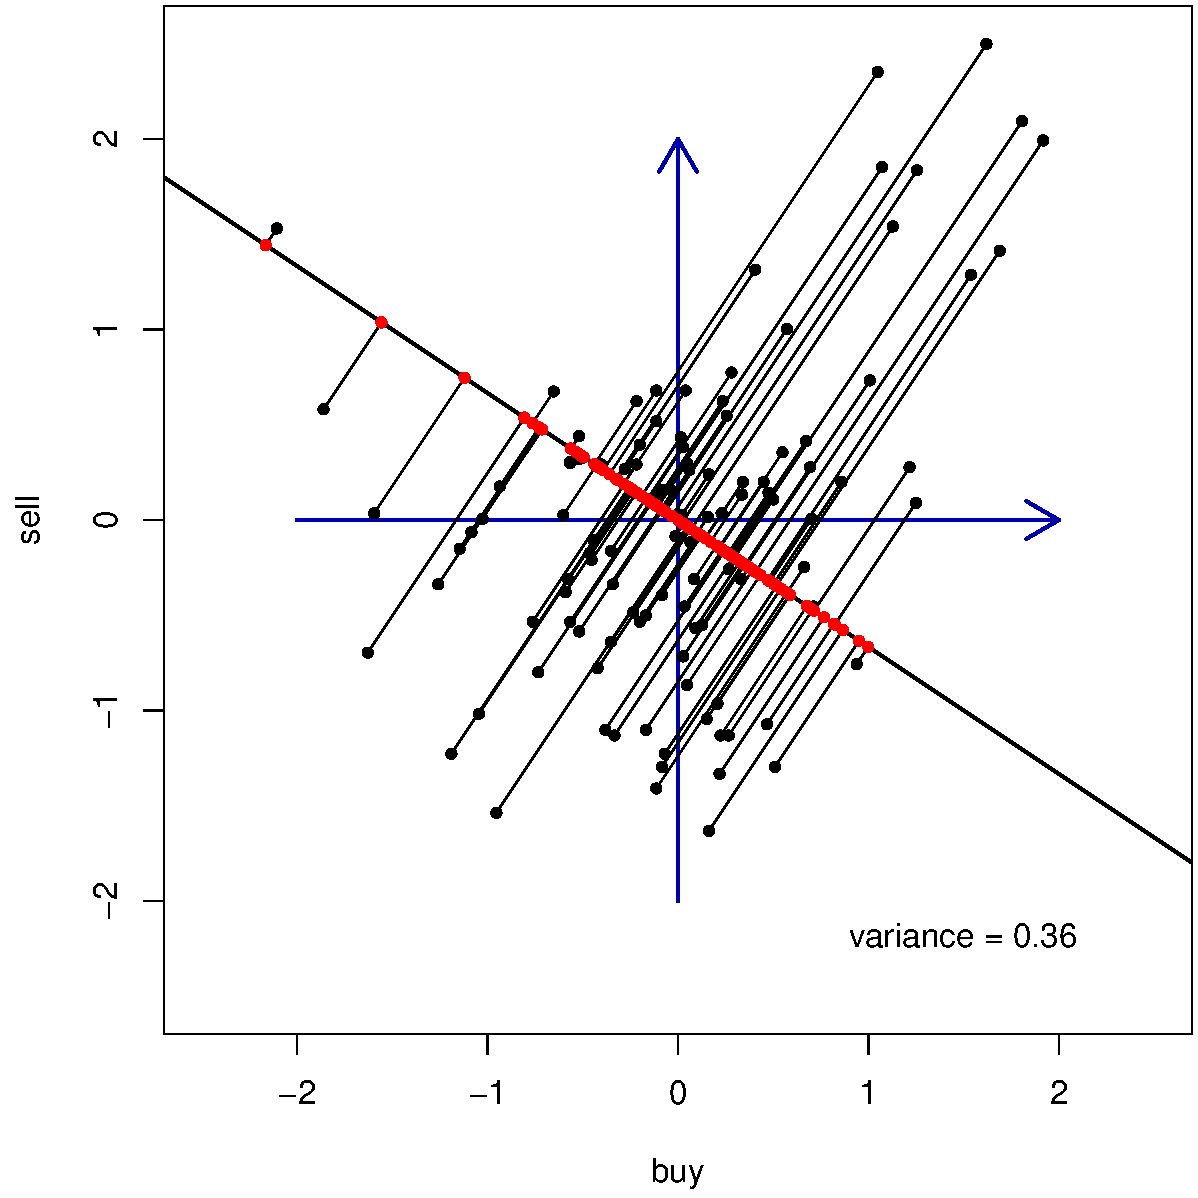
\includegraphics[width=7cm]{img/3_buy_sell_1_projection}}%
    \only<beamer:3| handout:0>{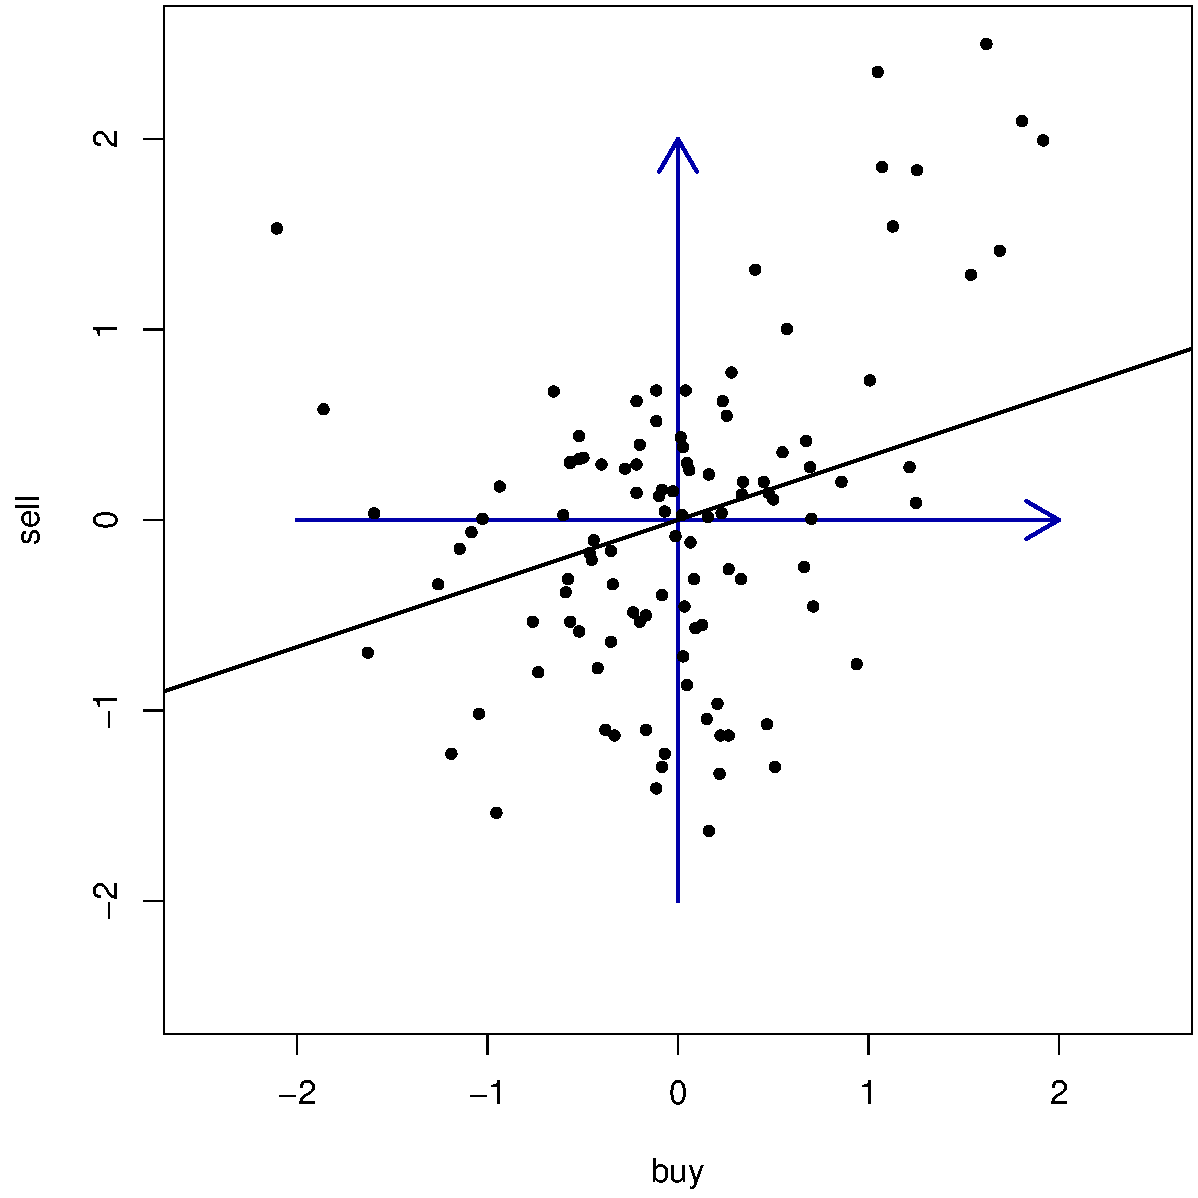
\includegraphics[width=7cm]{img/3_buy_sell_2_axis}}%
    \only<beamer:4| handout:2>{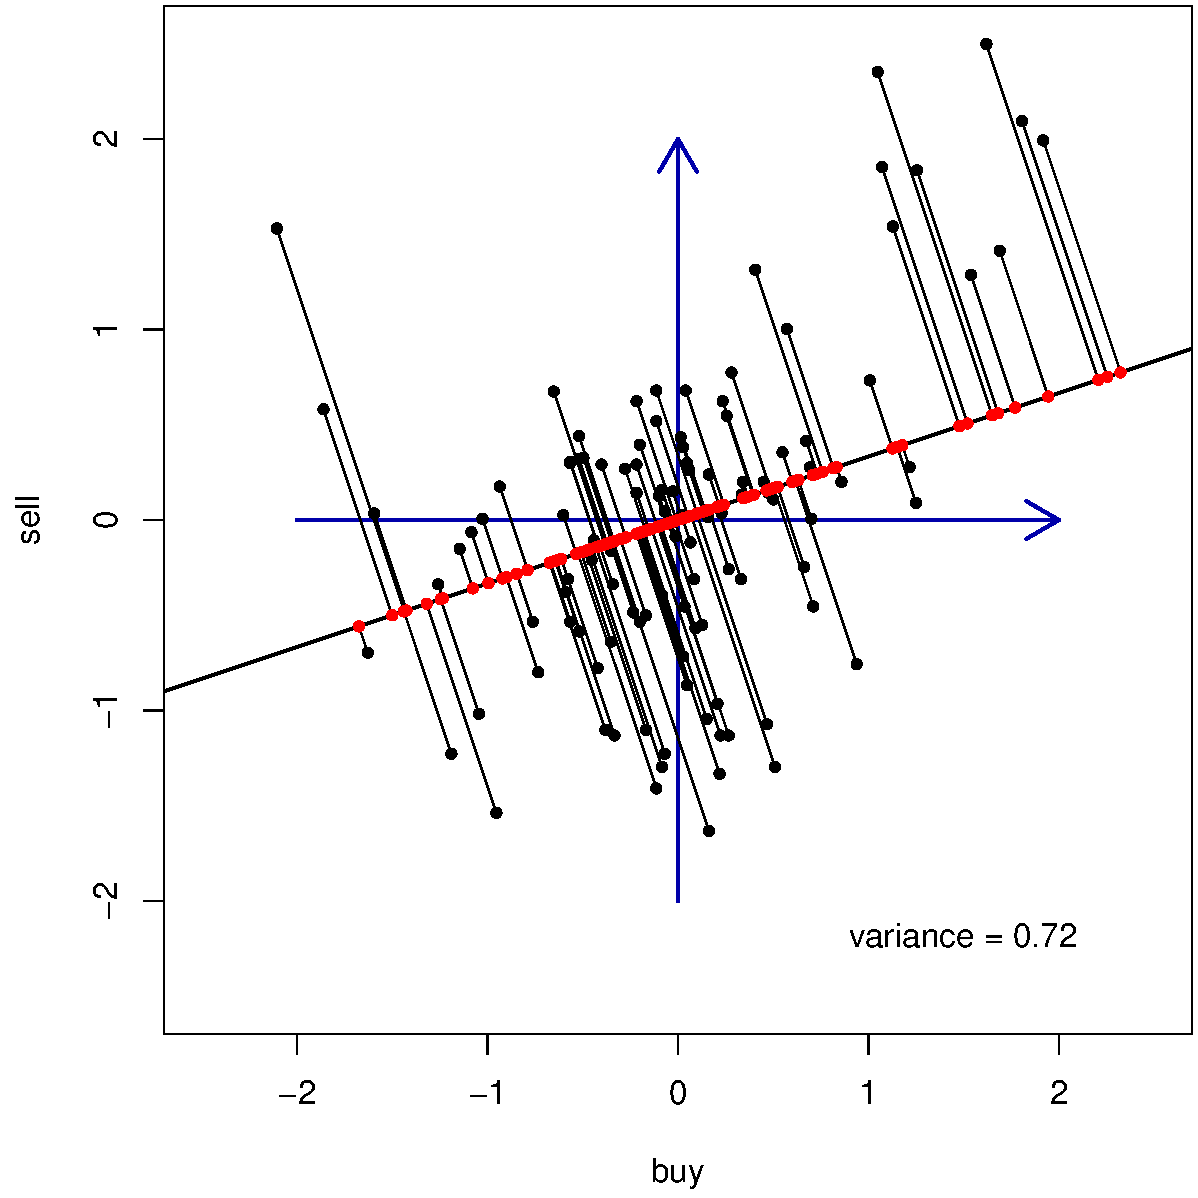
\includegraphics[width=7cm]{img/3_buy_sell_2_projection}}%
    \only<beamer:5| handout:0>{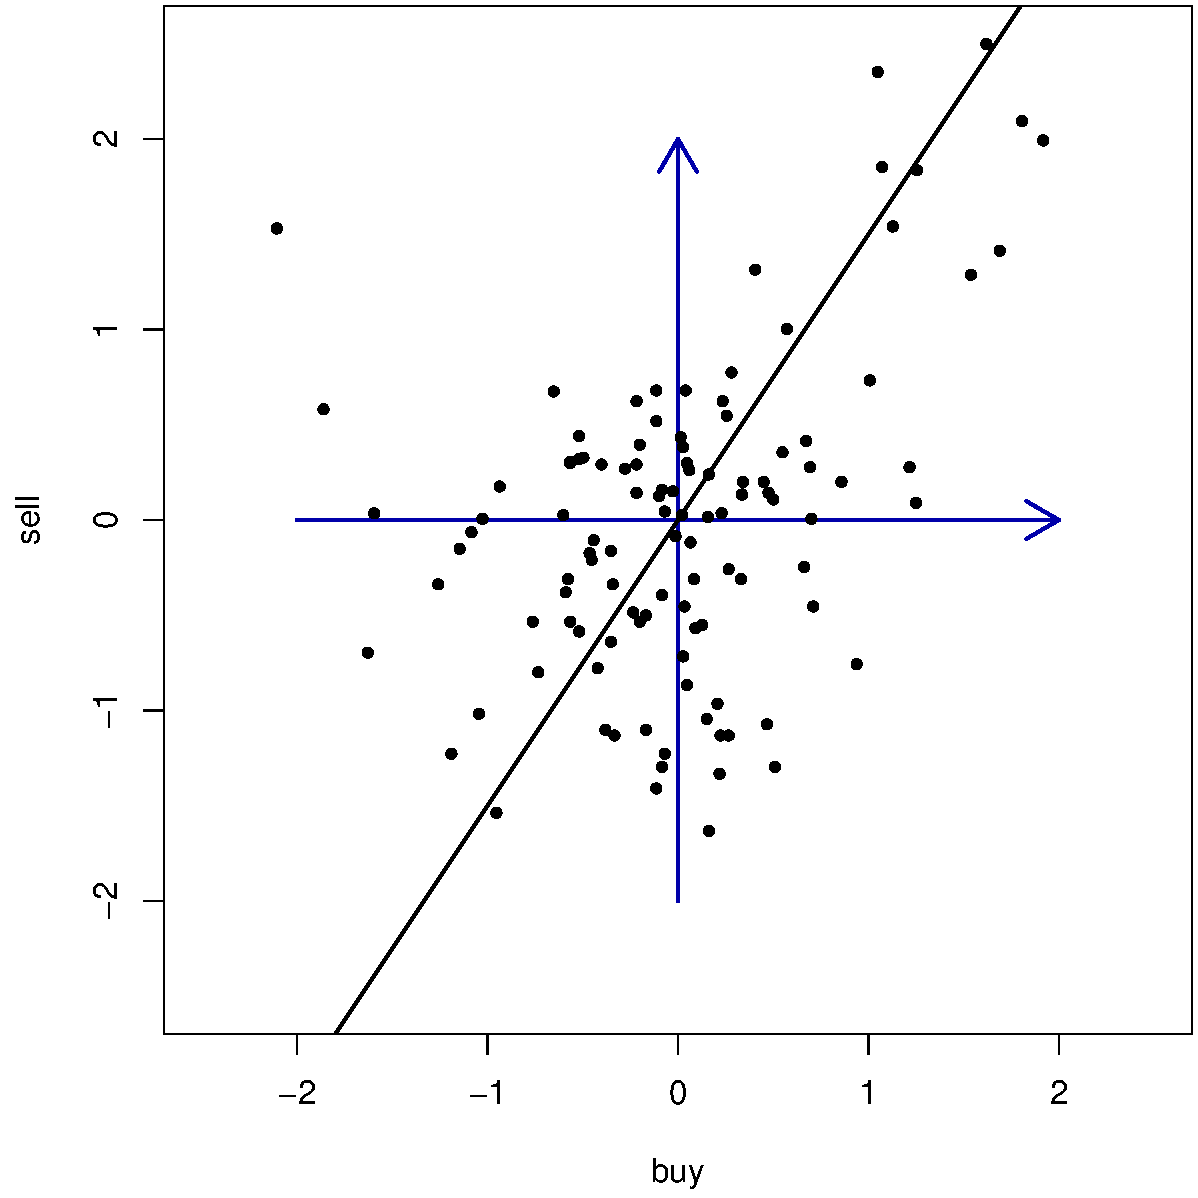
\includegraphics[width=7cm]{img/3_buy_sell_3_axis}}%
    \only<beamer:6| handout:3>{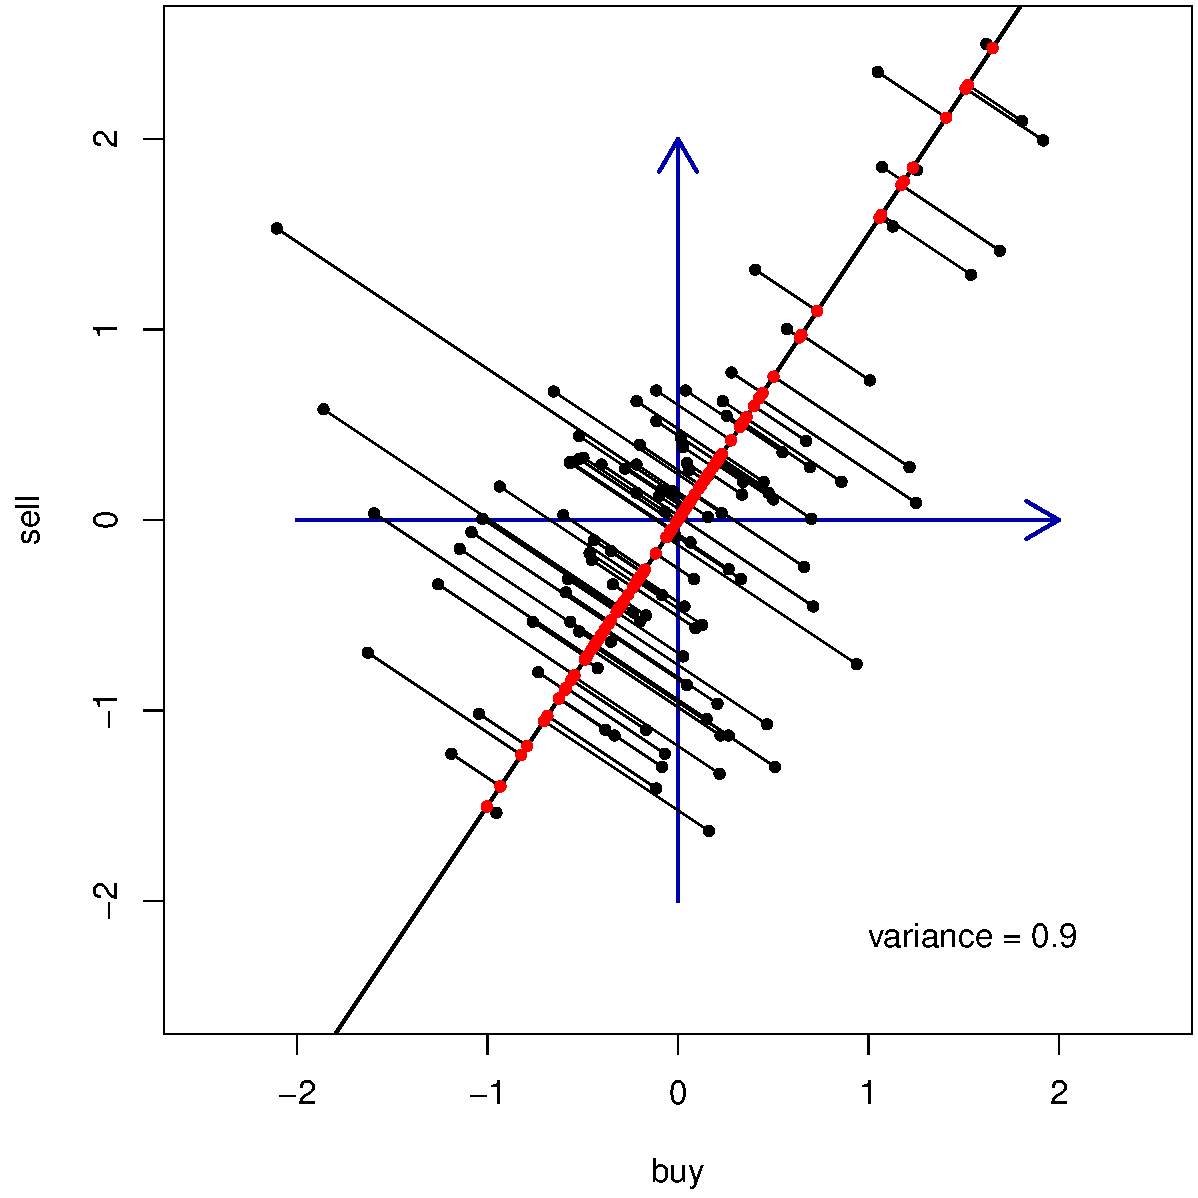
\includegraphics[width=7cm]{img/3_buy_sell_3_projection}}%
  \end{center}
\end{frame}

\begin{frame}
  \frametitle{The mathematics of projections}
  %% \framesubtitle{}

  \begin{columns}[c]
    \begin{column}{50mm}
      \begin{itemize}
      \item Line through origin given by unit vector
        $\norm{\vv} = 1$
      \item For a point $\vx$ and the corresponding unit vector $\vx' = \vx /
        \norm{\vx}$, we have \( \cos \varphi = \sprod{\vx'}{\vv} \)
      \end{itemize}
    \end{column}
    \begin{column}{50mm}
      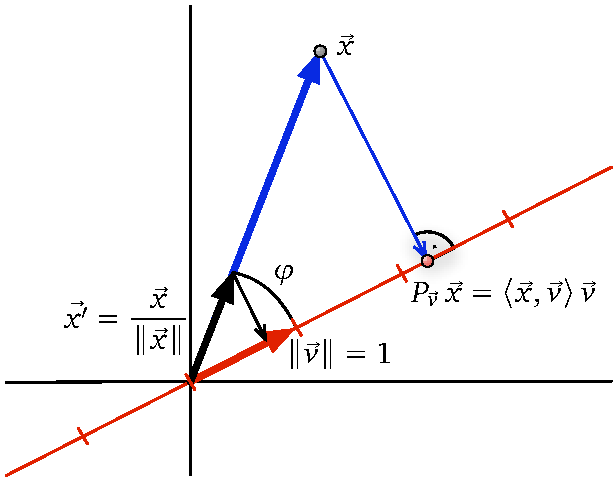
\includegraphics[width=50mm]{img/3_cosine_projection}
    \end{column}
  \end{columns}
  
  \pause
  \begin{itemize}
  \item Trigonometry: position of projected point on the line is
    $\norm{\vx}\cdot \cos\varphi = \norm{\vx}\cdot \sprod{\vx'}{\vv} =
    \sprod{\vx}{\vv}$
%  \item (projected point in original space is $\sprod{\vx}{\vv} \vv$)
  \item Preserved variance = one-dimensional variance on the line
    (note that data set is still centered after projection)
    \[
    \sigma_{\vv}^2 = \frac{1}{k-1} \sum_{i=1}^k \sprod{\vx_i}{\vv}^2
    \]
  \end{itemize}
\end{frame}

%%% Local Variables: 
%%% mode: latex
%%% TeX-master: "../../workspace"
%%% End: 
